\documentclass[12pt,a4paper]{article}

\usepackage{fontspec}
\usepackage{amsmath,amssymb,amsthm}
\usepackage{mathtools}
\usepackage{geometry}
\usepackage{hyperref}
\usepackage{microtype}
\usepackage{booktabs}
\usepackage{array}
\usepackage{xcolor}
\usepackage{tikz}
\usepackage{pgfplots}
\pgfplotsset{compat=1.18}
\usetikzlibrary{arrows.meta,positioning,decorations.pathreplacing,shapes.geometric,calc}
\usepackage{caption}
\usepackage{subcaption}
\usepackage{titlesec}
\usepackage{setspace}
\usepackage{parskip}
\usepackage{listings}

\geometry{
  top=1.25in,
  bottom=1.25in,
  left=1.35in,
  right=1.35in
}

\setmainfont{DejaVu Serif}
\setsansfont{DejaVu Sans}
\setmonofont{DejaVu Sans Mono}[Scale=0.82]

\definecolor{draftblue}{HTML}{1a3a5c}
\definecolor{draftgray}{HTML}{4a4a4a}
\definecolor{draftrule}{HTML}{8aadca}
\definecolor{codebg}{HTML}{f4f6f8}
\definecolor{codekey}{HTML}{1a3a5c}
\definecolor{codestr}{HTML}{2e6b3e}
\definecolor{codecom}{HTML}{7a7a7a}

\hypersetup{
  colorlinks=true,
  linkcolor=draftblue,
  citecolor=draftblue,
  urlcolor=draftblue,
  pdftitle={Draft-Net: Trajectory Learning for Stochastic Revision and Spectral Refinement},
  pdfauthor={Flyxion}
}

\lstset{
  basicstyle=\ttfamily\small,
  backgroundcolor=\color{codebg},
  keywordstyle=\color{codekey}\bfseries,
  stringstyle=\color{codestr},
  commentstyle=\color{codecom}\itshape,
  breaklines=true,
  frame=single,
  framesep=4pt,
  rulecolor=\color{draftrule},
  xleftmargin=8pt,
  xrightmargin=8pt,
  language=Python,
  showstringspaces=false
}

\titleformat{\section}{\large\bfseries\color{draftblue}}{\thesection.}{0.6em}{}[\vspace{0.1em}\color{draftrule}\hrule\vspace{0.2em}]
\titleformat{\subsection}{\normalsize\bfseries\color{draftgray}}{\thesubsection.}{0.5em}{}
\titleformat{\subsubsection}{\normalsize\itshape\color{draftgray}}{\thesubsubsection.}{0.4em}{}

\newtheoremstyle{draftthm}
  {0.7em}{0.5em}{\itshape}{}{\bfseries\color{draftblue}}{.}{0.5em}{}
\theoremstyle{draftthm}
\newtheorem{definition}{Definition}[section]
\newtheorem{theorem}{Theorem}[section]
\newtheorem{proposition}{Proposition}[section]
\newtheorem{remark}{Remark}[section]

\newcommand{\D}{\mathcal{D}}
\newcommand{\Lat}{\mathbb{R}^{m}}
\newcommand{\traj}{\gamma}
\newcommand{\enc}{E}
\newcommand{\vtheta}{v_{\theta}}
\newcommand{\Ftheta}{F_{\theta}}
\newcommand{\Gtheta}{G_{\theta}}
\newcommand{\norm}[1]{\left\|#1\right\|}
\newcommand{\ptheta}{p_{\theta}}
\newcommand{\dz}{\Delta z}
\newcommand{\bW}{W}
\newcommand{\code}[1]{\texttt{\small #1}}

\begin{document}

% ---------------------------------------------------------------
% TITLE PAGE
% ---------------------------------------------------------------
\begin{titlepage}
\centering
\vspace*{1.8cm}

{\color{draftblue}\rule{\linewidth}{1.4pt}}\\[0.4em]
{\color{draftblue}\rule{\linewidth}{0.4pt}}

\vspace{1.0cm}
{\fontsize{22}{28}\selectfont\bfseries\color{draftblue}
Draft-Net: Trajectory Learning for\\[0.25em]
Stochastic Revision and Spectral Refinement}

\vspace{0.9cm}
{\color{draftblue}\rule{0.5\linewidth}{0.4pt}}

\vspace{0.8cm}
{\large Flyxion}

\vspace{0.4cm}
{\normalsize\color{draftgray}\itshape Independent Scholar}

\vspace{0.6cm}
{\small\color{draftgray} \today}

\vspace{1.2cm}
{\color{draftblue}\rule{\linewidth}{0.4pt}}\\[0.2em]
{\color{draftblue}\rule{\linewidth}{1.4pt}}

\vspace{1.4cm}
\begin{minipage}{0.88\textwidth}
\small\itshape\color{draftgray}
\textbf{Abstract.}\quad
Traditional generative models focus on the probability of a final artifact, collapsing the history of human creation into a singular distributional event. Draft-Net proposes a shift toward learning the trajectory $\traj(t)$, treating documents and images as paths through a high-dimensional latent manifold rather than static samples. By training on version-controlled empirical data---Git commit histories, manuscript revision sequences, and layered painting progress shots---Draft-Net learns the vector fields of authorial intent. The framework departs from autoregressive models in two fundamental respects: it conditions generation on both initial and terminal states, formulating intermediate reconstruction as a stochastic bridge problem; and it employs a dyadic iterative resolution curriculum that progressively increases the temporal granularity of the learned trajectory. The architecture extends to the visual domain through spectral decomposition, in which low-frequency compositional structures are established before high-frequency edges and highlights emerge. Integration with the Relativistic Scalar-Vector Plenum framework augments each draft state with scalar density, directional flow, and informational entropy diagnostics. Path-fidelity metrics replace perplexity as the primary evaluation criterion. The reference implementation is organized as a Python package, \texttt{draftnet}, providing five CLI entry points, modular encoders, a bridge predictor, a velocity estimator, an image spectral module, and a suite of trajectory evaluation functions.
\end{minipage}

\vspace{1.0cm}
{\small\color{draftgray}
\textit{Keywords}: trajectory learning, stochastic revision, Schrödinger bridge, spectral refinement,
RSVP field theory, version-controlled corpora, path fidelity, latent manifolds}
\end{titlepage}

% ---------------------------------------------------------------
\setstretch{1.18}
\tableofcontents
\newpage

% ---------------------------------------------------------------
\section{Introduction: From Static Likelihood to Dynamic Evolution}
% ---------------------------------------------------------------

\subsection{The Limits of Endpoint Modeling}

Modern generative models are primarily trained to approximate the probability of a final artifact. In language modeling this takes the canonical form of next-token prediction, where a model learns

\begin{equation}
  P_{\theta}(w_i \mid w_{<i}).
\end{equation}

Image generators learn a mapping from a noise distribution to a final image. In both cases the training objective orients entirely toward reproducing a terminal state. The trajectory through which an artifact emerges---its drafts, revisions, structural reorganizations, and iterative refinements---is discarded as training signal.

This compression is computationally tractable and empirically powerful. It also constitutes a systematic loss of information. The intermediate states of a creative process contain evidence of intention, uncertainty, self-correction, and structural reasoning that is invisible in the final product alone.

\subsection{The Trajectory Hypothesis}

Human creative practice is inherently temporal. Authors write rough drafts, reorganize arguments, compress redundant passages, and refine style across multiple iterations. Painters begin with broad compositional blocking before introducing form, shadow, and highlight. Programmers refactor code over dozens of commits, each representing a local decision about structure or abstraction. In each domain the final artifact is only the terminal point of a trajectory of transformations.

The central hypothesis of this work is therefore: intelligence in creative domains is better characterized as the ability to navigate transformation paths than as the ability to produce terminal states. Rather than learning $P(x)$, a capable model should learn the trajectory $\traj(t)$ through which artifacts evolve.

\subsection{From Token Prediction to Revision Prediction}

The conceptual transition is a change in the conditioning structure of the generative objective. Standard autoregressive models condition only on prior context. Draft-Net instead conditions on both the current state and the terminal goal:

\begin{equation}
  P_{\theta}(d_{t+1} \mid d_t, d_T),
\end{equation}

where $d_t$ is the current draft and $d_T$ is the finished work. The model is not predicting what word comes next in a distribution over arbitrary text; it is predicting what revision step comes next in the trajectory from a particular rough beginning to a particular finished artifact.

\subsection{Contributions}

The framework introduced here makes the following contributions. It defines a formal representation of draft trajectories and their embedding into latent manifolds. It presents a stochastic bridge formulation for learning revision dynamics between fixed endpoints. It introduces a dyadic resolution curriculum that progressively increases temporal granularity. It extends the trajectory framework to the visual domain through Fourier spectral decomposition. It incorporates RSVP field diagnostics as augmented latent state variables. It proposes path-fidelity metrics as principled replacements for perplexity. And it provides a reference implementation, described in detail in Section~\ref{sec:implementation}, as a fully structured Python package.

% ---------------------------------------------------------------
\section{Formal Foundations of Draft Trajectories}
% ---------------------------------------------------------------

\subsection{The Manifold of Creative Artifacts}

Let $\D$ denote the space of all possible creative artifacts. In the textual case $\D$ consists of all finite token sequences over a vocabulary $\mathcal{V}$; in the visual case it consists of all images on a fixed canvas; in the code domain it consists of all syntactically well-formed programs. In each case the space is discrete at the symbol level but admits meaningful continuous structure at the semantic level.

\begin{definition}[Artifact Manifold]
  Let $\D$ be a set of creative artifacts equipped with a dissimilarity measure $\mathrm{dist}: \D \times \D \to \mathbb{R}_{\geq 0}$. An \emph{artifact manifold} is a continuous space $\mathcal{M}$ together with an encoder $\enc: \D \to \mathcal{M}$ that embeds artifacts into a metric space with smooth interpolation properties.
\end{definition}

Throughout this paper $\mathcal{M} = \Lat$ for a fixed dimensionality $m$, and $z = \enc(d)$ denotes the latent representation of a draft $d$.

\subsection{Draft Sequences and Trajectories}

\begin{definition}[Draft Sequence]
  A \emph{draft sequence} is an ordered tuple
  \begin{equation}
    D = (d_0, d_1, \dots, d_T)
  \end{equation}
  where $d_0$ is an initial rough artifact and $d_T$ is the finished work. The sequence represents the empirical revision history of a single artifact.
\end{definition}

A draft sequence induces a trajectory in latent space via the encoder. Define

\begin{equation}
  z_t = \enc(d_t), \qquad z_t \in \Lat.
\end{equation}

The discrete latent sequence $(z_0, z_1, \dots, z_T)$ is a sampling of a continuous trajectory $\traj: [0,T] \to \Lat$.

In the reference implementation, the type \code{DraftTrajectory} (\code{draftnet/types.py}) realizes this definition directly:

\begin{lstlisting}
@dataclass
class DraftTrajectory:
    trajectory_id: str
    modality: Modality          # "text" | "code" | "latex" | "image"
    source: str
    states: List[DraftState]    # ordered D = (d_0, ..., d_T)
    metadata: Dict[str, Any] = field(default_factory=dict)
\end{lstlisting}

Each \code{DraftState} carries \code{content\_path}, \code{content\_hash}, optional \code{latent}, \code{diff\_from\_prev}, and \code{rsvp} field summaries, providing the complete per-step annotation required by the training pipeline.

\subsection{The Revision Velocity Field}

The local dynamics of revision are described by the \emph{edit velocity}:

\begin{equation}
  \dz_t = z_{t+1} - z_t.
\end{equation}

This discrete difference approximates the continuous derivative

\begin{equation}
  \frac{dz}{dt} = v(z, t),
\end{equation}

which is a vector field over the latent manifold. The training objective for Draft-Net can be stated as learning this vector field from empirical trajectory data.

\begin{definition}[Transformation Operator]
  The local \emph{transformation operator} at time $t$ is the map $\Delta_t: \D \to \D$, implemented as a structured diff over the artifact. For text, $\Delta_t$ decomposes into insertions, deletions, and substitutions. The function \code{diff\_summary} (\code{draftnet/extract/diffs.py}) computes this decomposition, returning inserted, deleted, and replaced character counts together with a full unified diff string.
\end{definition}

% ---------------------------------------------------------------
\section{Stochastic Revision and Bridge Processes}
% ---------------------------------------------------------------

\subsection{Human Revision as a Stochastic Process}

Revision is guided but not deterministic. Even when an author knows the destination of their work, local editing decisions vary across realizations of the same general trajectory. An author rewriting a paragraph does not follow a unique path from initial to final form; many paths are plausible, and the realized path represents one sample from a distribution over revision behaviors.

\subsection{Stochastic Differential Equation Formulation}

\begin{definition}[Revision SDE]
  The revision dynamics in latent space are modeled by the stochastic differential equation
  \begin{equation}
    dz_t = \vtheta(z_t, t)\, dt + \sigma(t)\, d\bW_t,
    \label{eq:revision-sde}
  \end{equation}
  where $\vtheta(z_t, t)$ is a learned drift vector field representing directional revision intent, $\sigma(t) \geq 0$ is a time-dependent exploration noise coefficient, and $\bW_t$ is a standard Wiener process.
\end{definition}

The drift term encodes what the model learns about the direction of improvement. The noise term represents the stochastic component of local editing decisions.

\subsection{Endpoint-Conditioned Revision Bridges}

Unlike standard diffusion models, which condition generation on an initial noise state, Draft-Net conditions revision on both the initial draft $d_0$ and the terminal artifact $d_T$. This transforms the learning problem into bridge estimation.

\begin{definition}[Revision Bridge]
  The \emph{revision bridge} is the conditional distribution
  \begin{equation}
    \ptheta(z_t \mid z_0, z_T, t)
  \end{equation}
  over latent states at time $t$ given the latent representations of the initial and final drafts.
\end{definition}

This formulation is related to the Schrödinger bridge problem: finding the stochastic process with fixed marginal distributions at $t=0$ and $t=T$ that minimizes a relative entropy cost. The training objective follows directly:

\begin{equation}
  \mathcal{L}_{\mathrm{bridge}}
  =
  \sum_{t=1}^{T-1}
  \norm{\hat{z}_t - z_t}^2,
  \label{eq:bridge-l2}
\end{equation}

where $\hat{z}_t = f_{\theta}(z_0, z_T, t)$ is the model's predicted intermediate state. The \code{bridge\_loss} function (\code{draftnet/losses/bridge\_loss.py}) implements this as mean squared error over the predicted and target latent vectors.

The bridge predictor itself is \code{BridgeMLP} (\code{draftnet/models/bridge.py}):

\begin{lstlisting}
class BridgeMLP(nn.Module):
    def forward(self, z0, zT, t) -> Tensor:
        te = self.time_proj(t)          # learned time embedding
        x  = torch.cat([z0, zT, te], dim=-1)
        return self.net(x)              # predicts z_hat_t
\end{lstlisting}

The model concatenates $z_0$, $z_T$, and a two-layer GELU-activated time projection, then decodes through a three-layer MLP with dropout. This architecture makes the endpoint conditioning structurally explicit.

\subsection{Iterative Resolution Curriculum}

The training procedure follows a dyadic curriculum that progressively increases the temporal resolution of the learned trajectory.

\begin{definition}[Dyadic Resolution Curriculum]
  At training stage $n$, the model reconstructs latent states at fractional times
  \begin{equation}
    t_k^{(n)} = \frac{k}{2^n} T, \qquad k = 1, 2, \dots, 2^n - 1.
  \end{equation}
  The loss at stage $n$ is
  \begin{equation}
    \mathcal{L}^{(n)}
    =
    \sum_{k=1}^{2^n - 1}
    \norm{\hat{z}_{t_k^{(n)}} - z_{t_k^{(n)}}}^2.
    \label{eq:dyadic-loss}
  \end{equation}
\end{definition}

The function \code{dyadic\_targets} (\code{draftnet/trajectories/subdivision.py}) implements this computation, returning a list of \code{(fractional\_time, state\_index)} pairs for a given trajectory length and curriculum level. The curriculum level is exposed as a hyperparameter in all training configurations.

\begin{figure}[h]
\centering
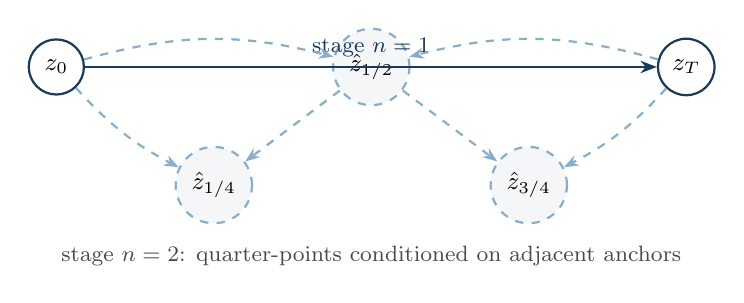
\begin{tikzpicture}[
  node distance=2.2cm,
  state/.style={circle, draw=draftblue, thick, fill=white, minimum size=0.7cm, font=\small},
  pred/.style={circle, draw=draftrule, thick, fill=codebg, minimum size=0.7cm, font=\small, dashed},
  arr/.style={-{Stealth[scale=0.9]}, draftblue, thick},
  parr/.style={-{Stealth[scale=0.8]}, draftrule, thick, dashed}
]
\node[state] (z0) at (0,0) {$z_0$};
\node[state] (zT) at (8,0) {$z_T$};
\node[pred]  (z12) at (4,0) {$\hat z_{1/2}$};
\node[pred]  (z14) at (2,-1.5) {$\hat z_{1/4}$};
\node[pred]  (z34) at (6,-1.5) {$\hat z_{3/4}$};

\draw[arr] (z0) -- node[above,font=\footnotesize]{stage $n=1$} (zT);
\draw[parr] (z0) to[bend left=15] (z12);
\draw[parr] (zT) to[bend right=15] (z12);
\draw[parr] (z0) to[bend right=10] (z14);
\draw[parr] (z12) -- (z14);
\draw[parr] (z12) -- (z34);
\draw[parr] (zT) to[bend left=10] (z34);

\node[font=\footnotesize,color=draftgray] at (4,-2.4) {stage $n=2$: quarter-points conditioned on adjacent anchors};
\end{tikzpicture}
\caption{Dyadic curriculum. At level $n=1$ the model predicts the midpoint $\hat z_{1/2}$ from the endpoint pair. At level $n=2$ the quarter-points are predicted using the midpoint as an additional conditioning anchor. Each successive level doubles the temporal resolution.}
\label{fig:dyadic}
\end{figure}

\subsection{Edit Velocity Supervision}

Beyond state reconstruction, the model can be trained to predict the direction of revision at each step. The \emph{revision increment} is

\begin{equation}
  \dz_t = z_{t+1} - z_t,
\end{equation}

and the velocity estimator $g_{\theta}$ is trained under

\begin{equation}
  \mathcal{L}_{\mathrm{vel}}
  =
  \sum_t
  \norm{g_{\theta}(z_t, z_T, t) - \dz_t}^2.
  \label{eq:velocity-loss}
\end{equation}

\code{VelocityMLP} (\code{draftnet/models/velocity.py}) accepts the concatenation of $z_t$, $z_T$, and $t$ and outputs the predicted revision direction. Velocity supervision is important because two trajectories may pass through similar latent regions while exhibiting qualitatively different local editing behavior---one compressive, another expansive---which the state alone does not distinguish.

% ---------------------------------------------------------------
\section{RSVP Integration: Field Diagnostics for Revision Dynamics}
% ---------------------------------------------------------------

\subsection{Framework Overview}

The Relativistic Scalar-Vector Plenum (RSVP) framework characterizes evolving structured systems through three coordinate fields: a scalar density measuring local informational concentration, a directional vector field capturing the flow of meaning or structure, and an entropy field measuring disorder. When applied to creative artifacts these fields provide interpretable diagnostics of revision dynamics that augment the geometric latent representation.

\subsection{Scalar Density, Vector Flow, and Entropy}

\begin{definition}[Scalar Density]
  Let $d$ be a text artifact tokenized over vocabulary $\mathcal{V}$, with $P(w)$ the empirical frequency of token $w$ in a reference corpus. The \emph{scalar density} of patch $p_i \subseteq d$ is
  \begin{equation}
    \Phi_i = \frac{1}{|p_i|} \sum_{w \in p_i} \bigl(-\log P(w)\bigr).
    \label{eq:scalar-density}
  \end{equation}
\end{definition}

In the implementation, \code{scalar\_density} (\code{draftnet/encoders/rsvp\_features.py}) approximates $\Phi$ as the product of mean token length and type-to-token ratio---a corpus-free proxy that is monotone in true information content. The function \code{vector\_flow} estimates directional progression by counting verbal action indicators and transitional discourse markers normalized by line count. Token Shannon entropy $S = -\sum_w p(w) \log p(w)$ is computed by \code{token\_entropy} over the full word distribution.

All three quantities are assembled by \code{rsvp\_features}, which returns a dictionary $\{\Phi, v, S\}$ for any text string. These values are used by \code{TextStatsEncoder} to prepend field diagnostics to the front of the hashed bag-of-words embedding, making the RSVP state visible to downstream models without requiring a separate field-augmented architecture.

\subsection{Augmented Latent State}

The full RSVP-augmented latent representation of a draft is

\begin{equation}
  x_t = (z_t,\, \Phi_t,\, \mathbf{v}_t,\, S_t),
  \label{eq:augmented-state}
\end{equation}

and revision dynamics in the augmented state space are governed by

\begin{equation}
  dx_t = \Ftheta(x_t, t)\, dt + \Gtheta(x_t, t)\, d\bW_t.
  \label{eq:augmented-sde}
\end{equation}

The entropy reduction hypothesis---that finished artifacts have lower entropy than initial drafts, $S(d_T) < S(d_0)$---is empirically testable from the stored \code{rsvp} field in each \code{DraftState}, and can be enforced as a training-time regularization constraint in the \code{rsvp\_augmented.yaml} configuration.

% ---------------------------------------------------------------
\section{Draft-Net for Textual Revision}
% ---------------------------------------------------------------

\subsection{Dataset Construction and Git Extraction}

Training requires corpora in which artifacts appear in multiple successive versions. Three sources provide this structure: Git commit histories from software and writing repositories, \LaTeX{} manuscript revision histories, and Wikipedia revision logs.

The extraction pipeline is implemented in \code{draftnet/extract/git.py}. The function \code{build\_trajectory\_from\_git} enumerates commits in chronological order, decodes the file content at each commit hash, applies optional \LaTeX{} normalization through \code{TexNormalizationConfig}, writes each state to disk, computes the diff summary against the prior state, and assembles the complete \code{DraftTrajectory}. The \code{TexNormalizationConfig} dataclass (\code{draftnet/extract/tex.py}) controls three normalization passes: comment stripping, whitespace collapsing, and include flattening.

The \code{draftnet-extract} CLI entry point accepts a YAML configuration file specifying \code{repo\_path}, \code{file\_globs}, output directories, and normalization options. The \code{tex\_revision.yaml} configuration is preconfigured for \code{*.tex} file extraction with normalization disabled by default.

\subsection{Edit Operators and the Diff Representation}

The transformation operator between consecutive text drafts decomposes into insertions, deletions, and substitutions. The \code{diff\_summary} function (\code{draftnet/extract/diffs.py}) uses Python's \code{difflib.SequenceMatcher} to count character-level edit operations and stores a full unified diff alongside the character counts. The structural statistics function \code{structural\_stats} (\code{draftnet/extract/tex.py}) additionally counts \LaTeX{} structural markers---sections, subsections, equations, citations, and figures---providing document-level trajectory diagnostics.

\subsection{Training Objective}

The full training loss combines the bridge reconstruction loss, the velocity loss, and an optional RSVP field alignment term:

\begin{equation}
  \mathcal{L}
  =
  \lambda_1 \mathcal{L}_{\mathrm{bridge}}
  +
  \lambda_2 \mathcal{L}_{\mathrm{vel}}
  +
  \lambda_3 \mathcal{L}_{\mathrm{field}},
  \label{eq:combined-loss}
\end{equation}

where $\lambda_1, \lambda_2, \lambda_3 \geq 0$ are hyperparameters. The standard training loop (\code{draftnet/cli/train.py}) minimizes $\mathcal{L}_{\mathrm{bridge}}$ alone by default; the additional terms can be introduced by extending the training script with velocity and field alignment losses, both of which are fully implemented in \code{draftnet/losses/}.

% ---------------------------------------------------------------
\section{Draft-Net for Vision: Spectral Painting Trajectories}
% ---------------------------------------------------------------

\subsection{Painting as a Frequency Evolution}

Painting evolves through a predictable hierarchy of spatial frequencies. Painters trained in the classical atelier tradition first establish large compositional masses before introducing medium-scale forms, and finally add high-frequency edges, texture, and highlights. This hierarchy mirrors the logic of visual construction, in which global relationships must be established before local details can be correctly placed.

\subsection{Fourier Representation and Spectral Energy}

\begin{definition}[Fourier Transform of a Painting]
  The spatial Fourier transform of image $I_t$ is
  \begin{equation}
    \hat{I}_t(u,v) = \int\!\!\int I_t(x,y)\, e^{-2\pi i(ux+vy)}\, dx\, dy.
  \end{equation}
\end{definition}

The \emph{spectral energy} in band $k$ at stage $t$ is

\begin{equation}
  E_k(t) = \int\!\!\int \bigl|\hat{I}_t(u,v)\bigr|^2 B_k(u,v)\, du\, dv.
  \label{eq:spectral-energy}
\end{equation}

The function \code{spectral\_band\_energies} (\code{draftnet/utils/image\_ops.py}) implements this computation without any heavy dependencies: it constructs radial frequency masks via \code{radial\_frequency\_masks}, computes the 2D FFT of the luminance channel using \code{numpy.fft.fft2}, computes the power spectrum $|\hat{I}|^2$, integrates over each band mask, and returns the band energies normalized to unit sum. Low-$k$ bands capture large compositional structures; high-$k$ bands capture fine edges and texture.

\subsection{Logistic Growth Model}

Empirically, the spectral energy of each band follows a logistic growth curve over the painting trajectory:

\begin{equation}
  E_k(t) = \frac{A_k}{1 + e^{-a_k(t - t_k)}},
  \label{eq:logistic-growth}
\end{equation}

with the ordering constraint $t_1 < t_2 < \cdots < t_K$ encoding the principle that low-frequency structure precedes high-frequency detail. The spectral training loss is

\begin{equation}
  \mathcal{L}_{\mathrm{spec}}
  =
  \sum_{k,t}
  \bigl(\hat{E}_k(t) - E_k(t)\bigr)^2,
  \label{eq:spectral-loss}
\end{equation}

implemented as \code{spectral\_loss} (\code{draftnet/losses/spectral\_loss.py}) with optional per-band weights for scale-aware training.

\subsection{Laplacian Pyramid Decomposition}

The coarse-to-fine pyramid decomposition provides a spatially interpretable alternative to the Fourier representation. Define the low-pass approximation as $L_0 = \mathrm{LowPass}(I)$ and detail layers as $L_{k+1} = I_k - \mathrm{Upsample}(L_k)$, so that

\begin{equation}
  I = L_0 + L_1 + \cdots + L_K.
\end{equation}

The function \code{coarse\_to\_fine\_pyramid} (\code{draftnet/utils/image\_ops.py}) generates this decomposition using a box blur as the low-pass operator, with blur radius decreasing across levels. The painting evolution is parameterized as

\begin{equation}
  I_t = \sum_{k=0}^{K} \alpha_k(t)\, L_k,
\end{equation}

with the temporal coefficients $\alpha_k(t)$ growing over time. The \code{reverse\_spectral\_plan} function (\code{draftnet/models/spectral.py}) uses the pyramid to estimate the likely painting construction order from a finished image, producing a sequence of progressively coarser approximations that trace the plausible reverse workflow.

% ---------------------------------------------------------------
\section{Object-Layered Composition Dynamics}
% ---------------------------------------------------------------

\subsection{Foreground-Background Segmentation}

In figurative painting the canvas partitions naturally into background regions and foreground objects that resolve later in the process. Draft-Net formalizes this through a segmentation mask.

\begin{definition}[Segmentation Field]
  Let $M(x,y) \in [0,1]$ be a continuous foreground mask. The image decomposes as
  \begin{equation}
    I(x,y) = (1-M)\, I_{\mathrm{bg}} + M\, I_{\mathrm{fg}}.
    \label{eq:image-decomp}
  \end{equation}
\end{definition}

The function \code{segmentation\_mask} (\code{draftnet/utils/image\_ops.py}) produces a soft luminance-threshold mask, with a fallback to contrast-based segmentation when the luminance threshold produces a degenerate partition. The function \code{estimate\_foreground\_mask} (\code{draftnet/models/segmentation.py}) wraps this for use in the composition model.

\subsection{Blurred Foreground and Temporal Schedules}

At early painting stages foreground regions are replaced by Gaussian-blurred placeholders:

\begin{equation}
  I^{(\mathrm{early})} = (1-M)\, I_{\mathrm{bg}} + M\, G_{\sigma}(I),
  \label{eq:early-image}
\end{equation}

implemented by \code{apply\_soft\_foreground\_blur} (\code{draftnet/utils/image\_ops.py}). The blurred foreground carries approximate hue and value without edges or fine texture, allowing background gradients to extend continuously across figure boundaries.

As the trajectory progresses the blur radius decays exponentially:

\begin{equation}
  \sigma(t) = \sigma_0\, e^{-\lambda t}.
  \label{eq:blur-schedule}
\end{equation}

The foreground influence weight grows according to a logistic schedule:

\begin{equation}
  w_{\mathrm{fg}}(t) = \frac{1}{1 + e^{-a(t - t_0)}},
  \label{eq:fg-weight}
\end{equation}

implemented as \code{foreground\_schedule} (\code{draftnet/models/segmentation.py}), parameterized by a midpoint $t_0$ and steepness $a$. The early-stage composite is assembled by \code{early\_stage\_composite}, which returns the blended image together with the estimated mask.

\subsection{Compositional Update Rule}

The painting update at each trajectory step is

\begin{equation}
  \Delta I_t = (1-M)\, \Delta I_{\mathrm{bg}} + w_{\mathrm{fg}}(t)\, M\, \Delta I_{\mathrm{fg}},
  \label{eq:update-rule}
\end{equation}

so that early in the trajectory background development dominates and late in the trajectory foreground refinement dominates. The complete six-stage protocol that emerges from combining equations \eqref{eq:early-image}, \eqref{eq:blur-schedule}, \eqref{eq:fg-weight}, and \eqref{eq:update-rule} formalizes the classical atelier method as a learned temporal schedule directly recoverable from image progress data.

% ---------------------------------------------------------------
\section{Reverse Trajectory Planning}
% ---------------------------------------------------------------

\subsection{Inverting the Velocity Field}

The learned velocity field $\vtheta(z_t, t)$ can be integrated backward in time to reconstruct a plausible history of a finished artifact. Given the terminal state $z_T$, the backward recursion is

\begin{equation}
  z_{t-1} = z_t - \vtheta(z_t, t)\, \Delta t.
  \label{eq:backward-integration}
\end{equation}

The \code{draftnet-reverse} CLI entry point (\code{draftnet/cli/reverse.py}) implements this, iterating backward through fractional time steps and printing the resulting latent sequence as JSON. For the spectral domain, \code{reverse\_spectral\_plan} produces the equivalent sequence by recursively extracting lower-frequency approximations of the final image.

\subsection{Applications}

Reverse trajectory planning recovers the construction order of a finished artifact. In painting pedagogy the reverse trajectory reveals the likely order of operations used by an artist, which can be reconstructed as a step-by-step instructional sequence. In manuscript analysis the backward integration exposes the structural skeleton underlying a finished essay. In code analysis it can identify the abstract architectural decisions from which a complex implementation was progressively derived.

% ---------------------------------------------------------------
\section{Performance Evaluation}
% ---------------------------------------------------------------

\subsection{Inadequacy of Perplexity}

Standard language model evaluation uses perplexity, measuring how well the model assigns probability to held-out token sequences from the terminal distribution. Perplexity is orthogonal to trajectory fidelity. For Draft-Net the relevant question is not whether the model can produce plausible final artifacts, but whether its predicted trajectories match the structure of real authorial histories.

\subsection{Path Error and Edit Path Distance}

The primary scalar evaluation metric is \emph{Path Error}:

\begin{equation}
  \mathrm{PE}(\hat\traj, \traj)
  =
  \sum_{t=1}^{T-1}
  \norm{\hat{z}_t - z_t}^2.
  \label{eq:path-error}
\end{equation}

Implemented by \code{path\_error} (\code{draftnet/trajectories/path\_metrics.py}) and wrapped by \code{path\_fidelity} (\code{draftnet/eval/fidelity.py}), which returns both the raw squared error and the bounded score $1/(1+\mathrm{PE})$.

The \emph{Edit Path Distance} evaluates fidelity in artifact space rather than latent space:

\begin{equation}
  \mathrm{EPD}(\hat\traj, \traj)
  =
  \sum_{t=1}^{T-1}
  \mathrm{EditDist}(\hat{d}_t, d_t),
  \label{eq:epd}
\end{equation}

where \code{edit\_distance} (\code{draftnet/eval/edit\_distance.py}) computes $1 - \mathrm{SequenceMatcher.ratio}(a, b)$, giving a normalized dissimilarity in $[0,1]$. The \code{edit\_path\_loss} function (\code{draftnet/losses/edit\_path\_loss.py}) sums this over a batch of predicted-and-target text pairs.

\subsection{RSVP Field Alignment}

\begin{equation}
  \mathrm{FieldErr}(\hat\traj, \traj)
  =
  \sum_{t=1}^{T-1}
  \Bigl(
  |\hat\Phi_t - \Phi_t|
  + \norm{\hat{\mathbf{v}}_t - \mathbf{v}_t}
  + |\hat{S}_t - S_t|
  \Bigr),
  \label{eq:field-error}
\end{equation}

implemented by \code{field\_alignment} (\code{draftnet/eval/field\_alignment.py}), which returns the mean absolute error for each of the three RSVP fields separately.

\subsection{Combined Selection Score}

Model selection uses a weighted combination:

\begin{equation}
  \mathrm{Score}(\theta)
  =
  \lambda_1\, \mathrm{PE}
  +
  \lambda_2\, \mathrm{EPD}
  +
  \lambda_3\, \mathrm{FieldErr}.
  \label{eq:combined-score}
\end{equation}

The \code{draftnet-eval} CLI runs inference over the held-out trajectory set and reports \code{path\_error} and \code{path\_fidelity}; EPD and field alignment can be added to the evaluation loop using the provided loss and evaluation utilities.

% ---------------------------------------------------------------
\section{Implementation and Data Pipelines}
\label{sec:implementation}
% ---------------------------------------------------------------

\subsection{Package Structure}

The reference implementation is organized as the \code{draftnet} Python package with the following top-level submodules:

\begin{center}
\begin{tabular}{ll}
\toprule
Submodule & Content \\
\midrule
\code{types} & \code{DraftState}, \code{DraftTrajectory}, \code{Modality} \\
\code{extract} & Git extraction, diff computation, \LaTeX{} normalization, image ingestion \\
\code{encoders} & Base class, text stats encoder, image stats encoder, RSVP features \\
\code{trajectories} & Draft utilities, dyadic subdivision, path metrics \\
\code{data} & Schema, manifest I/O, text and image \code{Dataset} classes, batch collation \\
\code{models} & Bridge MLP, velocity MLP, reverse planner, spectral model, segmentation \\
\code{losses} & Bridge, velocity, edit-path, and spectral losses \\
\code{eval} & Path fidelity, edit distance, field alignment, reconstruction metrics \\
\code{utils} & File I/O (JSONL, YAML, text), SHA-256 hashing, distance metrics, image ops \\
\code{cli} & Five entry points: extract, train, eval, replay, reverse \\
\bottomrule
\end{tabular}
\end{center}

\subsection{CLI Workflow}

The standard workflow proceeds through four CLI commands:

\begin{lstlisting}
# 1. Extract trajectories from a Git repository
draftnet-extract --config configs/tex_revision.yaml

# 2. Train the bridge model with curriculum level 2
draftnet-train  --config configs/text_bridge.yaml

# 3. Evaluate path fidelity on held-out trajectories
draftnet-eval   --config configs/text_bridge.yaml \
                --checkpoint experiments/bridge.pt

# 4. Replay or reverse-plan a single trajectory
draftnet-replay  --config configs/text_bridge.yaml \
                 --checkpoint experiments/bridge.pt \
                 --trajectory tex_paper_001
draftnet-reverse --config configs/text_bridge.yaml \
                 --checkpoint experiments/bridge.pt \
                 --steps 16
\end{lstlisting}

\subsection{Configuration System}

All hyperparameters are controlled through YAML configuration files that support a single level of inheritance via the \code{base\_config} key, merged by \code{resolve\_config} (\code{draftnet/cli/common.py}). The repository ships five configurations:

\begin{center}
\begin{tabular}{ll}
\toprule
File & Purpose \\
\midrule
\code{base.yaml} & Shared defaults (seed, encoder dim, model size, optimizer) \\
\code{text\_bridge.yaml} & Text bridge training at curriculum level 2 \\
\code{tex\_revision.yaml} & Git extraction for \code{*.tex} files \\
\code{painting\_spectral.yaml} & Image bridge training, 64-dim encoder, 4 spectral bands \\
\code{rsvp\_augmented.yaml} & Curriculum level 3 with RSVP field augmentation \\
\bottomrule
\end{tabular}
\end{center}

\subsection{Image Pipeline}

For the visual domain, \code{extract\_painting\_progress.py} walks a directory of per-painting subdirectories, discovers image files with \code{.npy}, \code{.npz}, \code{.ppm}, or \code{.pgm} extensions, and calls \code{build\_image\_trajectory} to construct a \code{DraftTrajectory} with spectral and segmentation annotations at each state. The \code{ImageBridgeDataset} (\code{draftnet/data/image\_loader.py}) encodes each image through \code{ImageStatsEncoder}, which extracts channel means, luminance statistics, edge statistics, foreground ratio, and normalized spectral band energies into a single fixed-length latent vector.

% ---------------------------------------------------------------
\section{Discussion}
% ---------------------------------------------------------------

\subsection{Relation to Diffusion Models}

Standard image diffusion models define a forward process that progressively corrupts a clean image toward Gaussian noise. Draft-Net differs in two important respects. First, the corruption direction in Draft-Net is semantically meaningful---moving from polished to rough corresponds to actual revision dynamics rather than arbitrary noise injection. Second, the model conditions on both endpoints, learning a bridge rather than a free denoising process. This changes the mathematical structure from a Markov chain conditioned on one endpoint to a stochastic process conditioned on two fixed marginals.

\subsection{Relation to Autoregressive Language Models}

Autoregressive models generate tokens left-to-right, conditioning each prediction on its full prior context. Draft-Net generates revision states forward in time, conditioning each intermediate state on both the initial draft and the terminal artifact. The key structural difference is the availability of the endpoint. Standard autoregressive models must generate into an unknown future; Draft-Net navigates a known destination. This transforms generation from an open-ended extrapolation into a constrained interpolation.

\subsection{Relation to Optimal Transport}

The bridge formulation connects directly to the theory of optimal transport. The initial and final drafts define two point masses in artifact space, and the revision process is a stochastic transport plan between the distributions $\mu_0$ and $\mu_T$ they induce. The Schrödinger bridge problem identifies the transport plan with minimum relative entropy; the empirical trajectories in the training corpus serve as noisy observations of this optimal plan. Draft-Net can therefore be viewed as a parametric estimator of the Schrödinger bridge between initial and final draft distributions, anchored in real authorial histories rather than synthetically constructed endpoints.

% ---------------------------------------------------------------
\section{Future Directions}
% ---------------------------------------------------------------

Several extensions are under investigation. Real-time collaborative revision systems could track the joint trajectory of multiple authors, learning how their individual editing fields interact and converge. Cross-domain trajectory transfer would test whether revision dynamics share universal geometric properties across creative modalities---whether the spectral hierarchy of painting, for instance, informs structural refinement in writing. Revision-style modeling would train separate velocity fields for different authors or editor profiles, enabling the model to emulate specific editorial voices. Integration with reinforcement learning would allow the trajectory framework to be extended toward active editing assistance, where the model learns not just to predict revisions but to suggest them under a user-defined reward signal.

The current implementation provides a concrete platform for each of these directions. The modular encoder architecture makes it straightforward to substitute transformer-based text encoders or vision transformer image encoders as stronger pretrained representations become available. The manifest-based data pipeline abstracts over data sources, so Wikipedia revision logs, digital painting layer histories, and software refactoring commit sequences can all be ingested through the same extraction interface.

% ---------------------------------------------------------------
\section{Conclusion}
% ---------------------------------------------------------------

This paper has introduced Draft-Net, a trajectory-learning framework that reframes generative modeling as process learning rather than endpoint generation. The central shift is from modeling the distribution of finished artifacts to modeling the latent geometry of creative revision. By training on version-controlled empirical histories, Draft-Net learns the vector fields that govern how documents and images move through their respective latent manifolds during authorial refinement.

The mathematical core comprises a stochastic differential equation model of revision dynamics, an endpoint-conditioned bridge formulation of intermediate state prediction, a dyadic iterative resolution curriculum, and RSVP field augmentation for interpretable diagnostic representation. The spectral extension to the visual domain formalizes the classical principle that large compositional structures precede fine detail in terms of Fourier frequency evolution and Laplacian pyramid decomposition. The object-layered composition model captures the atelier method's temporal structure as a learned schedule. The path-fidelity evaluation metrics provide a rigorous framework for selecting models by how faithfully their predicted trajectories reconstruct real authorial histories.

The reference implementation realizes all of these abstractions as a structured Python package with five CLI entry points, modular encoders, model components, losses, and evaluation utilities that are immediately usable on any version-controlled artifact corpus.

Taken together, these contributions define a geometry of creation: not the probability of what exists, but the dynamics of how things come to be.

% ---------------------------------------------------------------
\appendix
\section{Notation Summary}
% ---------------------------------------------------------------

\begin{center}
\begin{tabular}{ll}
\toprule
Symbol & Meaning \\
\midrule
$\D$ & Space of creative artifacts \\
$D = (d_0, \dots, d_T)$ & Draft sequence \\
$z_t = \enc(d_t)$ & Latent embedding of draft $t$ \\
$\traj(t)$ & Continuous trajectory in latent space \\
$\dz_t = z_{t+1}-z_t$ & Discrete revision velocity \\
$\vtheta(z,t)$ & Learned drift vector field \\
$\sigma(t)$ & Exploration noise coefficient \\
$\bW_t$ & Wiener process \\
$\ptheta(z_t \mid z_0, z_T, t)$ & Revision bridge distribution \\
$\Phi_t$ & Scalar density (RSVP) \\
$\mathbf{v}_t$ & Directional vector flow (RSVP) \\
$S_t$ & Informational entropy (RSVP) \\
$x_t = (z_t, \Phi_t, \mathbf{v}_t, S_t)$ & RSVP-augmented latent state \\
$E_k(t)$ & Spectral energy in band $k$ at stage $t$ \\
$M(x,y)$ & Foreground segmentation mask \\
$G_\sigma$ & Gaussian blur with scale $\sigma$ \\
$\sigma(t) = \sigma_0 e^{-\lambda t}$ & Temporal blur decay schedule \\
$w_{\mathrm{fg}}(t)$ & Foreground influence weight \\
$\mathrm{PE}$ & Path Error (latent squared distance) \\
$\mathrm{EPD}$ & Edit Path Distance (artifact-space) \\
$\mathrm{FieldErr}$ & RSVP field mean absolute error \\
\bottomrule
\end{tabular}
\end{center}

\section{Module Reference}
\label{sec:module-ref}

\begin{center}
\begin{tabular}{ll}
\toprule
Module path & Key symbols \\
\midrule
\code{draftnet/types.py} & \code{DraftState}, \code{DraftTrajectory}, \code{Modality} \\
\code{draftnet/extract/git.py} & \code{build\_trajectory\_from\_git} \\
\code{draftnet/extract/diffs.py} & \code{diff\_summary}, \code{unified\_diff} \\
\code{draftnet/extract/tex.py} & \code{normalize\_tex}, \code{structural\_stats} \\
\code{draftnet/extract/image\_progress.py} & \code{build\_image\_trajectory} \\
\code{draftnet/encoders/rsvp\_features.py} & \code{rsvp\_features}, \code{scalar\_density}, \code{vector\_flow}, \code{token\_entropy} \\
\code{draftnet/encoders/text\_encoder.py} & \code{TextStatsEncoder} \\
\code{draftnet/encoders/image\_encoder.py} & \code{ImageStatsEncoder} \\
\code{draftnet/trajectories/subdivision.py} & \code{dyadic\_targets} \\
\code{draftnet/trajectories/path\_metrics.py} & \code{path\_error} \\
\code{draftnet/models/bridge.py} & \code{BridgeMLP} \\
\code{draftnet/models/velocity.py} & \code{VelocityMLP} \\
\code{draftnet/models/planner.py} & \code{replay\_bridge} \\
\code{draftnet/models/spectral.py} & \code{spectral\_summary}, \code{reverse\_spectral\_plan} \\
\code{draftnet/models/segmentation.py} & \code{early\_stage\_composite}, \code{foreground\_schedule} \\
\code{draftnet/losses/bridge\_loss.py} & \code{bridge\_loss} \\
\code{draftnet/losses/velocity\_loss.py} & \code{velocity\_loss} \\
\code{draftnet/losses/edit\_path\_loss.py} & \code{edit\_path\_loss} \\
\code{draftnet/losses/spectral\_loss.py} & \code{spectral\_loss} \\
\code{draftnet/eval/fidelity.py} & \code{path\_fidelity} \\
\code{draftnet/eval/edit\_distance.py} & \code{edit\_distance} \\
\code{draftnet/eval/field\_alignment.py} & \code{field\_alignment} \\
\code{draftnet/utils/image\_ops.py} & \code{spectral\_band\_energies}, \code{coarse\_to\_fine\_pyramid}, \code{apply\_soft\_foreground\_blur} \\
\bottomrule
\end{tabular}
\end{center}

\end{document}
